\documentclass[conference]{IEEEtran}
\usepackage{blindtext, graphicx}
\usepackage[spanish]{babel}
\usepackage{skmath}
\usepackage[utf8]{inputenc}
\usepackage{amsmath}
\usepackage{amsfonts}
\usepackage{graphicx}
\usepackage[colorinlistoftodos]{todonotes}
\usepackage{algorithm}
\usepackage{algpseudocode}
\usepackage{enumerate}
\begin{document}
\title{$II$ Segundo Proyecto Programado Backtracking}
\author{\IEEEauthorblockN{Daniel Alvarado Bonilla}
\IEEEauthorblockA{Instituto Tecnol\'ogico de Costa Rica\\Ingenier\'ia en Computaci\'on\\
2014089192\\
Email: daniel.alvarado.bonilla@gmail.com}
\and
\IEEEauthorblockN{Roberto Rojas Segnini}
\IEEEauthorblockA{Instituto Tecnol\'ogico de Costa Rica\\Ingenier\'ia en Computaci\'on\\
2016139072\\
Email: rojassegniniroberto@gmail.com}
}
\maketitle
\begin{abstract}
%\boldmath
%\blindtext[1]
ACA VA EL ABSTRACT
\end{abstract}
\begin{IEEEkeywords}
Big O, Matrix, Algorithm, Kakuro, Backtracking, Permutations.
\end{IEEEkeywords}
\section{Introducci\'on}
Existen muchi\'isimos tipos de algoritmos y un programador se define en cual tipo de algoritmo se escoge para resolver un determinado problema que tiene una variedad soluciones. Se debe entender el por qu\'e de la escogencia de este tipo. Es decir, en ocaciones no se quiere utilizar el algoritmo mas eficiente, esto no quiere decir que se tiene que utilizar un algoritmo mal fundamento, si no todo lo contrario, poder saber cuando se debe hacer uso de un algoritmo que no se basa en su eficiencia.\\
Un o de estos tipos de algoritmos es llamado Backtracking o "Vuelta Atras". Este algoritmo se basa en construir soluciones parciales a medida que se progresa en el arbol de opciones de nuestro problema.  En otras palabras es una t\'ecnica de programaci\'on para hacer una b\'usqueda sistem\'atica a tra\'aves de todas las posibles configuraciones de nuestro problema. Todos los algoritmos de backtracking siguen un mismo patr\'on, pero var\'ia un poco con el problema. \\Se puede observar su forma gen\'erica en la secci\'on de Pseudoc\'odigos.
\\
En el presente trabajo se investigo, trabajo para crear una pequeña aplicaci\'on con el fin de que este genere Kakuros.  Un kakuro es un enigma l\'ogico que es semejante al conocido Crucigrama. Pero este no usa letras ni palabras, si no, n\'umeros. Se les conoce tambi\'en como Suma Cruzada, es un juego bastante popular en Jap\'on. 
El algoritmo de backtracking explicado anteriormente es utilizado para resolver diferentes Kakuros. Para mejor la eficiencia del mismo, se inventaron diferentes algoritmos mas pequeños de "poda" para asi disminuir de manera significante el \'arbol de posibles soluciones.  Para las diferentes funciones se hizo un an\'alisis de O grande y se realizaron distintos experimentos.
\begin{figure}
	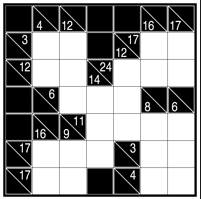
\includegraphics[scale=0.5]{kakuroImg.png}
	\caption{Kakuro}
\end{figure}
\section{Pseudoc\'odigo}
  \begin{algorithm}
   \caption{Backtracking  Generic Algorithm}
    \begin{algorithmic}[1]
      \Function{backTracking}{$v[1..k]$ }\\\Comment{v es un vector $k$prometedor}
		\\
        \State si v es una solucion entonces escribir v
        \For{ para cada vector$(k+1)-$prometedor w}
        \State tal que $w[1..k] = v[1..k]$
        \State hacer backTracking$(w[1..k+1])$
        \EndFor
       \EndFunction
\end{algorithmic}
\end{algorithm}

\begin{algorithm}
   \caption{Solve - Backtracking Algorithm implemented}
    \begin{algorithmic}[1]
      \Function{solveKakuro}{$kakuro$ }\\\Comment{kakuro es una matriz, la cual contiene el kakuro sin soluci\'on}
		\\
		\If{noEmptySpaces(kakuro)}
		    \If{isKakuroSolved(kakuro)}
		        \State return True
		    \Else
		    \EndIf
		        \State return False
 		 \Else
 		 \EndIf
		    \State position=getNextPosition(kakuro)
		    \State row=position[0]
		    \State column=position[1]
		    \State num1 = getNumberLeft(kakuro, position)
		    
		    \If{num1 == 0}
		        \State num1 = -25
		    \EndIf
		    \State num2 = getNumberUp(kakuro, position)
		    
		    \If{num2 == 0}
		        \State num2 = -25
		    \EndIf
		    
		    \State deleteRepeatedValues(kakuro,getIntersection
		    \State (getValues(kakuro,position,num1,num2),
		    \State getValuesList(num1,num2,kakuro,position)),position)
		    
		    \If{values==[]}
		        \State return False
		    \EndIf
		    
		    \For{i en el largo de values}
		        \State value = values[i]
		        \State kakuro[row][column] = value
		        \If{solveKakuro(kakuro)}
		            \State return True
		        \Else
		            \State kakuro[row][column] = BLANK\_ SPACE
		            \EndIf
		    \EndFor
		    
	\State return False

       \EndFunction
\end{algorithmic}
\end{algorithm}
  \begin{algorithm}
   \caption{substract Values Algorithm}
    \begin{algorithmic}[1]
      \Function{substractVal}{$k[1..k]$,$p[x,y] $,$sum$,$bool$ }\
        \State newSum = 0
        \State newSpaces = 0
        \If{left}
        		\State row = p[0]
        		\State col = p[1]
        		\While{col$ >= 0$}
        			\If{k[row][col] es vector}
        				\State spaces = getSpaces()
        				\State break
        			\EndIf
        			\State col$-$
        		\EndWhile
        		\State col $+ 1$
        	\EndIf
        	\For{i en rango de spaces}
        	\If{k[row][col$+i$]  tiene un valor entonces}
        		\State spaces $-= 1$
        		\State sum $-= $ [el valor que este en esa posici\'on]
        	\EndIf
        	\EndFor
        	\If{not left}
        		\State row = p[0]
        		\State col = p[1]
        		\While{col$ >= 0$}
        			\If{k[row][col] es vector}
        				\State spaces = getSpaces()
        				\State break
        			\EndIf
        			\State row$- 1$
        		\EndWhile
        		\State row $+ 1$
        	\EndIf
        	\For{i en rango de spaces}
        	\If{k[row$+i$][col]  tiene un valor entonces}
        		\State spaces $-= 1$
        		\State sum $-= $ [el valor que este en esa posici\'on]
        	\EndIf
        	\EndFor \\
		\Return sum,spaces
       \EndFunction
\end{algorithmic}
\end{algorithm}

  \begin{algorithm}
   \caption{Get Values Algorithm }
    \begin{algorithmic}[1]
      \Function{getValuesList}{$hSum$ $vSum$,$k[1..k]$,$p[x,y] $ }\
      \State  sumUp,spacesUp = substractValues(k,p,vSum,False)
      \State  sumLeft,spacesLeft = substractValues(k,p,hSum,True)
      \If{si el valor forma una suma vertical}
     	 	\If{spacesUp = 1}
     	 			\If{Si es una intersecci\'on de dos sumas}
     	 				\Return [sumUp]
     	 			\EndIf
     	 	\If{spacesLeft =1}
     	 			\If{si ambas sumas son iguales}
     	 					\State \Return [sum]
     	 			\Else
     	 			 		\State \Return vac\'io
     	 			\EndIf
     	 	\Else
     	 			\State combinaciones = getCombinations()
     	 			\Comment retorna un vector de combinacinoes que vienen de un diccionario	
     	 			\If{sumUp esta en combinaciones}
     	 					\State \Return [min de sumLeft y sumUp] si no []
     	 			\EndIf
     	 	\EndIf
     	 \Else
     	 		\State combinaciones = getCombinations()
     	 		\For{por combinacion en combinaciones]}
     	 			\State Agregar cada valor a un 
     	 			\State vector llamado valoresUp
     	 		\EndFor
     	 \EndIf
     \If{el valor forma una suma horizontal}
          	 	\If{SpacesLeft = 1}
     	 			\If{Si es una intersecci\'on de dos sumas}
     	 				\Return [sumLeft]
     	 			\EndIf
     	 	\If{SpacesUp =1}
     	 			\If{si ambas sumas son iguales}
     	 					\State \Return [sum]
     	 			\Else
     	 			 		\State \Return vac\'io
     	 			\EndIf
     	 	\Else
     	 			\State combinaciones = getCombinations()
     	 			\Comment retorna un vector de combinacinoes que vienen de un diccionario	
     	 			\If{sumUp esta en combinaciones}
     	 					\State \Return [min de sumLeft y sumUp] si no []
     	 			\EndIf
     	 	\EndIf
     	 \Else
     	 		\State combinaciones = getCombinations()
     	 		\For{por combinacion en combinaciones]}
     	 			\State Agregar cada valor a un 
     	 			\State vector llamado valoresLeft
     	 		\EndFor
     	 \EndIf
     	 \EndIf
      \EndIf
      \State \Return intersecci\'on entre valoresLeft y valoresRight
       \EndFunction
\end{algorithmic}
\end{algorithm}




\section{Complejidad de los Algoritmos}
Orden de $O(f(n))$ dde Funcion de Poda:\\
Este algoritmo tiene en s\'i bastantes funciones  pequeñas. Cada una siendo fundamental para la funci\'on de poda. Las m\'as relevantes se explicar\'an a continuaci\'on son:\\
\begin{enumerate}[I]
\item SubstractVal() es una funci\'on que toma el lugar donde se puede colocar un valor$[1..9]$, recibe tambi\'en este valor que se utilizar\'a las sumas a las que pertenece, el mejor caso es que sea una intersecci\'on de dos sumas, asi la lista de valores seria menor. Toma esta posici\'on y se mueve ya sea de forma vertical u horizontal, hasta buscar la suma a la que pertenece esa posici\'on. Al encontrar el vector $v[sumaVertical,sumaHorizontal]$ se desplaza contando los espacios disponibles que tiene esta suma.  Esto es un comportamiento lineal, es decir $O(n)$ al recorrer una lista. Lo interesante de este algoritmo es que una vez obtenida la cantidad de espacios, se recorre de nuevo desde la posici\'on en la que se encuentra el vector v mencionado anteriormente, y suma los las casillas que ya tienen  un valor. Y por cada casilla que tenga un valor, se aumenta un contador llamado newSpaces. Este es otro comportamiento lineal, es decir hasta el momento es un $O(2n)$. Este paso es sumamente importante, por que resta a la suma que se tiene que llegar, lo que se tiene hasta el momento. En otras palabras, si se debe llegar a sumar un total de $27$ en cuatro espacios, y ya se tiene $2$ espacios utilizados, se toman los valores de estos dos espacios, se suman y luego se le restan al $27$. Si se ten\'ia $3$ y $7$ la nueva suma a la que se tiene que llegar es $17$. Por \'ultimo este numero y los espacios nuevos  $(2)$ son retornados. Hasta el momento se tiene $O(2n)$. \\
Ver Algoritmo 3. 
\item La funci\'on getValuesList es aquella que interpreta los valores retornados por substractVal(). Este primero revisa si dicha posici\'on donde se colocar\'a el valor es intersecci\'on de una suma en forma vertical y/o forma horizontal. Si pertenece a alguna de las anteriores, se verifica si tiene y si solo un espacio disponible, se utiliza una pequeña funcion la cu\'al retorna de un diccionario creado, donde este de llaves la cantidad de espacios disponibles, para cada de estas llaves tiene una llave secundaria la cual es la suma que puede formarse. Por \'ultimo, tiene un vector de vectores con las posibles combinaciones de valores para obtener esta suma en dicha cantidad de espacios.  Al obtenerla, se verifica que la suma, la cual es el unico valor que puede colocarse en la posici\'on dada, si no esta en estas combinaciones, se hace backtracking. Retorna una lista vac\'ia, donde el algoritmo principal ve que no tiene opciones que utilizar y se devuelve. Si la cantidad de espacios es diferente a uno, usando la funci\'on que obtiene las combinaciones, se agregan todos los valores posibles a una lista. Esto se hace para cada suma, siempre y cuando la posici\'on en la que se encuentra el algoritmo sea intersecci\'onTodo lo dicho anteriormente es de un orden lineal, sumando $O(2n + n)$. Esta funci\\on retorna este vector con los posibles valores que pueden ser utilizados y as\'i la funci\'on principal pruebe con estos.\\
Ver Algoritmo 4.
\end{enumerate}
El orden de la funci\'on de poda es de $O(n)$ ya que $3$ es una constante que no afecta el comportamiento de dicha funci\'on.
\\
Orden de $O(f(n))$ de Permutaciones:\\
FALTA
\\
Orden de $O(f(n))$ de Backtracking:\\
El algoritmo de Backtracking implementado se deduce que tiene un orden $O(n^k)$. $N$ es la cantidad de opciones que pueden colocarse en un determinado espacio del Kakuro. Al ser un \'arbol de soluciones, $N$ el nivel del nodo,  donde cada nodo tiene sus propios nodos, esto implica $n(n-1)(n-2)...(n-k+1)$. O grande considera el peor de los casos y este seria recorrer cada nodo hasta su ultimo nivel, es decir recorrer el \'arbol a profundidad. Siendo un comportamiento de $n^k$. Existe una funci\'on la cual recorre la matriz del Kakuro para encontrar una posici\'on libre, esta parte es $O(n^2)$. En total, $O(n^k + n^2)$ pero al como O Grande utiliza el peor de los casos, se concluye $O(n^k)$


\section{Experimentos}
\subsection{Experimento 1}


\begin{thebibliography}{1}

\bibitem{IEEEhowto:kopka}
H.~Kopka and P.~W. Daly, \emph{A Guide to \LaTeX}, 3rd~ed.\hskip 1em plus
  0.5em minus 0.4em\relax Harlow, England: Addison-Wesley, 1999.

\end{thebibliography}


\end{document}